%%%%%%%%%%%%%%%%%%%%%%%%%%%%%%%%%%%%%%%%%%%%%%%%%%%%%%%%%%%%%%%%%%%%%%%%%%%%%%%
%                     Heriot-Watt University Thesis Template  
%   Created by : Majed Al Saeed
%   Date:        June 2012
%   Department of Computer Science
%   Heriot-Watt University
%
%%%%%%%%%%%%%%%%%%%%%%%%%%%%%%%%%%%%%%%%%%%%%%%%%%%%%%%%%%%%%%%%%%%%%%%%%%%%%%%

\documentclass[a4paper,12pt]{report}


%==============================title page info=================================

% Name of the author
\newcommand{\auth}{Your Name}   
% Title of Thesis                
\newcommand{\thesistitle}{A Really Awesome University Guideline-Compliant Thesis}
% Degree  
\newcommand{\degree}{Doctor of Philosophy} 
% Date submitted
\newcommand{\supdate}{March 2013}            

%===================================packages===================================
\usepackage[top=20mm, bottom=20mm, left=40mm, right=20mm]{geometry}
\usepackage{setspace}
\usepackage{fancyhdr}
\usepackage[citecolor=black, urlcolor=black,
  linkcolor=black, colorlinks=true, bookmarksopen=false, bookmarks=true]{hyperref}
\usepackage[nonumberlist]{glossaries}
%Glossaries
\makeglossaries

% You must define terms or symbols before you can use them in the document. This is best done in the preamble. Each term is defined using:
% 
% \newglossaryentry{<label>}{<settings>}
% 
% where <label> is a unique label used to identify the term. The second argument, <settings>, is a key=value comma separated list that is used to set the required information for the term. A full list of available keys can be found in "Defining Glossary Entries" in the main glossaries user manual. The principle keys are name and description.
% 
% For example, to define the term "electrolyte":
% 
% \newglossaryentry{electrolyte}{name=electrolyte,
% description={solution able to conduct electric current}}
% 
% In the above example, the label and the name happen to be the same. In the next example, the name contains a ligature but the label doesn't:
% 
% \newglossaryentry{oesophagus}{name=\oe sophagus,
% description={canal from mouth to stomach},
%plural=\oe sophagi}

%\newacronym{<label>}{<abbrv>}{<full>}

%\gls{<label>}
%\glspl{<label>}

\newacronym{}{}{}

\newacronym{sisd}{SISD}{Single Instruction, Single Data} 

\newacronym{smp}{SMP}{shared memory multiprocessor}

\newacronym{ghc}{GHC}{Glasgow Haskell Compiler}

\newacronym{ghceden}{GHC-Eden}{The Parallel Haskell Compilation System Eden}

\newacronym{gph}{GpH}{Glasgow Parallel Haskell}

\newacronym{gdh}{GdH}{Glasgow Distributed Haskell}

\newacronym{ghcsmp}{GHC-SMP}{Haskell on a Shared Memory Multiprocessor}

\newacronym{hdph}{HdpH}{Haskell Distributed Parallel Haskell}

\newacronym{ghcpps}{GHC-PPS}{GHC Parallel Profiling System}

\newacronym{pe}{PE}{Processing Element}

\newacronym{uma}{UMA}{Uniform Memory Access}

\newacronym{numa}{NUMA}{Non-Uniform Memory Access}

\newacronym{mpp}{MPP}{Massively Parallel Processors}

\newacronym{mpi}{MPI}{Message Passing Interface}

\newacronym{pvm}{PVM}{Parallel Virtual Machine}

\newacronym{hpc}{HPC}{High-Performance Computing}

\newacronym{mcnoc}{McNoC}{Multicores Network-on-Chip}

\newacronym{api}{API}{Application Programming Interface} 


%\newacronym{}{}{}




\usepackage{graphicx}
\usepackage{subfigure}
\usepackage{xspace}
\usepackage{listings}
\usepackage{pdfpages}
\usepackage{alltt}
\usepackage{float} % to use [H] 
\usepackage[notindex, nottoc, notlof, notlot ]{tocbibind} 
%\usepackage{lscape}    % if you want to use land scape in one paper 
                       %...\begin{landscape}\end{landscape}

\setcounter{tocdepth}{3} 
\setcounter{secnumdepth}{3}

%===================================Document===================================
\begin{document}
\doublespacing

%==================================Title page==================================
\pagestyle{empty}
\begin{center}
\begin{spacing}{2}
{\large{\ \\  \vspace{1.5cm}\textbf{\MakeUppercase{\thesistitle}}}}\\
\end{spacing}
\vfill
{\Large\textit{by}}\\\vspace{0.2cm}
{\Large\upshape{\auth}}\\\vspace{1.0cm}

\includegraphics[width=3.5cm]{Figures/LogoBlack.jpg}\\
\vspace{1cm}
{\large Submitted for the degree of \\ \degree}\\
\vspace{1cm}
{\large\textsc{Department of Computer Science}\\
\textsc{School of Mathematical and Computer Sciences}\\
\textsc{Heriot-Watt University}}\vfill
{\large{\supdate}}
\end{center}
{\small The copyright in this thesis is owned by the author. Any quotation from the report or use of any of the information contained in it must acknowledge this report as the source of the quotation or information.}
%===================================Abstract===================================
\clearpage
\begin{center}
\LARGE\textbf {Abstract}
\end{center}
\vspace{1cm}

\begin{spacing}{1} 
\noindent
Write the abstract here.

In accordance with the Academic Regulations the thesis must contain an abstract preferably not exceeding 200 words, bound in to precede the thesis. The abstract should appear on its own, on a single page.  The format should be the sameas that of the main text. The abstract should provide a synopsis of the thesis and shall state clearly the nature and scope of the research undertaken and of the contribution made to the knowledge of the subject treated. There should be a brief statement of the method of investigation where appropriate, an outline of the major divisions or principal arguments of thework and a summary of any conclusions reached. The abstract must follow the Title Page.

Thesis guidelines can be found at: \\ \url{https://www.hw.ac.uk/uk/students/doc/guidelinesonsubmissionandformatofthesis.pdf }

\end{spacing}

%==================================frontmater==================================
\clearpage
\pagestyle{plain}
\clearpage\pagenumbering{roman}
\noindent
{\LARGE\textbf{Acknowledgements}}
\vspace{1cm}

\begin{spacing}{1} 
\noindent
write Acknowledgements here. 

After this comes the mandatory table of contents. 

\textbf{Lists of Tables and Figures, Glossary, List of Publications by the Candidate}

It is \textit{optional} to provide these lists. If provided, then they should start on the page following the table of contents and be in the order: Tables, Figures, Glossary (list of abbreviations), Publications.  

Items in lists of Tables and Figures should be in the order in which they occur in the text.
\end{spacing}

\tableofcontents
\listoftables
\listoffigures
% In order for the glossaries to appear you should run this command
% makeglossaries HWThesis
\printglossaries
%===================================headings===================================
\clearpage
\pagestyle{fancy}
\pagenumbering{arabic}
\fancyhead{}
\lhead{\slshape \leftmark} 
\cfoot{\thepage}
\renewcommand{\headrulewidth}{0.4pt}
\renewcommand{\footrulewidth}{0.0pt}
\renewcommand{\chaptermark}[1]{\markboth{\chaptername\ \thechapter:\ #1}{}}
%===================================Chapters===================================


\documentclass[../HWThesis.tex]{subfiles}
\begin{document}

\chapter{Introduction}
\label{ch:introduction}

For the Degree of Doctor of Philosophy the thesis shall not normally exceed 80,000 words and shall not normally exceed 400 pages in length including Appendices, with a limit of no more than 100,000 words. In exceptional circumstances, the Research Degrees Committee will consider requests for thesis exceeding 100,000 on a case by case basis. The number of pages of a thesis exceeding 80,000 words in length shall be increased on a pro rata basis in accordance with the word limit.  For the Degree of Doctor of Philosophy by Published Research, a critical review of the published research which shall be inthe range of 10,000 to 25,000 words must be submitted.

Chapter 1 of the thesis must be an Introduction, so headed, defining the relation of the thesis to other work in the same field and referring appropriately to any findings, propositions or new discoveries contained in the thesis and to any important points about sources or treatment.

Thesis guidelines can be found at: \\ \url{https://www.hw.ac.uk/uk/students/doc/guidelinesonsubmissionandformatofthesis.pdf }

Related documents and forms at: \url{https://www.hw.ac.uk/uk/students/studies/examinations/thesis.htm}

\section{Section}

\cite{ghc-pps}

\subsection{Subsection}

\subsubsection{Subsubsection}
\end{document}

\documentclass[../HWThesis.tex]{subfiles}
\begin{document}
\chapter{Background}
\label{ch:background}


\begin{figure}[H]
 \begin{center}
 \includegraphics [width=12cm]{Background/pic.png}
 \caption{Figure Caption.}
 \label{fig:label}
\end{center}
\end{figure} 

\cite{gum, ghc-smp}

\subsection{Subsection}

\begin{table}[H]
\begin{center}
\begin{tabular}{c c c c} % centered columns (4 columns)
\hline\hline %inserts double horizontal lines
Case & Method\#1 & Method\#2 & Method\#3 \\ [0.5ex] % inserts table 
%heading
\hline % inserts single horizontal line
1 & 50 & 837 & 970 \\ % inserting body of the table
2 & 47 & 877 & 230 \\
3 & 31 & 25 & 415 \\
4 & 35 & 144 & 2356 \\
5 & 45 & 300 & 556 \\ [1ex] % [1ex] adds vertical space
\hline %inserts single line
\end{tabular}\caption{Table Caption}
\label{tab:lable}
\end{center}
\end{table}


\subsubsection{Subsubsection}

\end{document}

\documentclass[../HWThesis.tex]{subfiles}
\begin{document}

\chapter{Design}
\label{ch:design}

Write..
\section{Section}

According to \cite{ghc-pps} ...


\begin{figure}[H]
 \begin{center}
 \includegraphics [width=12cm]{fig/Design/pic.png}
 \caption{Figure Caption.}
 \label{fig:label}
\end{center}
\end{figure} 


\subsection{Subsection}

\begin{table}[H]
\begin{center}
\begin{tabular}{c rrrrrrr} % creating eight columns
\hline\hline %inserting double-line
Audio Name&\multicolumn{7}{c}{Sum of Extracted Bits} \\ [0.5ex] 
\hline % inserts single-line
Police & 5 & -1 & 5& 5& -7& -5& 3\\ % Entering row contents
Midnight & 7 & -3 & 5& 3& -1& -3& 5\\
News & 9 & -3 & 7& 9& -5& -1& 9\\[1ex] % [1ex] adds vertical space
\hline % inserts single-line
\end{tabular}
\caption{Table Caption}
\label{tab:lable}
\end{center}
\end{table}


\subsubsection{Subsubsection}

\end{document}

\documentclass[../HWThesis.tex]{subfiles}
\begin{document}

\chapter{Conclusion and Future Work}
\label{ch:conclusion}
\end{document}



%===================================Appendix===================================
\appendix
\renewcommand{\chaptermark}[1]{\markboth{Appendix \thechapter.\ #1}{}}
\documentclass[../HWThesis.tex]{subfiles}
\begin{document}
\chapter{Foo}

Hi I'm an appendix

\end{document}

%=================================Bibliography=================================
\bibliographystyle{abbrv}
\bibliography{Bibliography}

\end{document}


